%!TEX root = ../thesis.tex

% \pagebreak[4]
% \hspace*{1cm}
% \pagebreak[4]
% \hspace*{1cm}
% \pagebreak[4]

\chapter{Extensions}

\graphicspath{ {Chapter4/Chapter4Figs/PNG/}
  {Chapter4/Chapter4Figs/PDF/} {Chapter4/Chapter4Figs/} }

Dans le dernier chapitre, nous avons vu une nouvelle méthode permettant
combiner des outils de déformation à base de cage. Cette méthode utilise un
nouveau type d'outil, la cage de contrôle d'influence. Cet outil est composé
de deux cages. L'une dite cage d'influence, elle délimite la zone de l'espace
sous l'influence de la déformation. L'autre dite de contrôle, elle permet à
l'utilisateur de contrôler la déformation à appliquer.

Ce sujet se tourne vers la création d'un outil multidimensionnel de
déformation. Mais nous n'avons pour l'instant travaillé que sur des
déformation à base d'outils de dimension 2. Il est naturel de se demander
comment notre méthode pourrait être étendue à des outils de dimensions
différentes. Deux approches sont possibles pour généraliser ce travail :

\begin{enumerate}
\item Modification de la nature de la cage de contrôle
\item Mélanger des outils existants avec cette méthode
\end{enumerate}

\section{Modification de la nature de la cage de contrôle}

Nous avions choisi de travailler avec une cage comme outil de contrôle puisque
nous voulions une méthode de mélange d'outils de déformation à base de cage.
Mais rien ne nous empêche de changer la nature de cette cage de contrôle. Pour
généraliser un peu plus ces propos, nommons la cage de contrôle \textit{outil
de contrôle}. A partir du moment où un outil (point, courbe, face) nous permet
de définir une cage d'influence (nécessaire aux méthodes d'atténuation et de
mélange), nous pouvons l'utiliser comme outil de contrôle.

Clarifions un peu ces explications. Imaginons que notre outil de contrôle soit
un point. Pour obtenir la cage d'influence associée à ce point, nous pouvons
construire un polygone régulier (de résolution quelconque) de façon à ce que
l'isobarycentre de ce polygone soit l'outil de contrôle (Figure \ref{EXTPoi}).
Le lien entre l'outil de contrôle et la cage d'influence s'établit sur le
principe que l'outil de contrôle doit rester l'isobarycentre de la cage
d'influence. La modification de la position de l'outil de contrôle implique
une modification de la position des sommets de la cage d'influence (par
invariance de l'association).

\begin{figure}[ht]
\begin{center}
  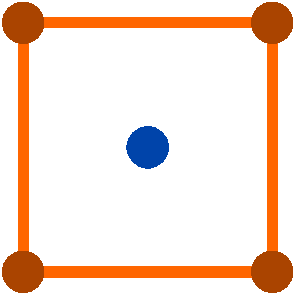
\includegraphics[scale=0.8]{chapter4-outilPoint4-pstricks}
  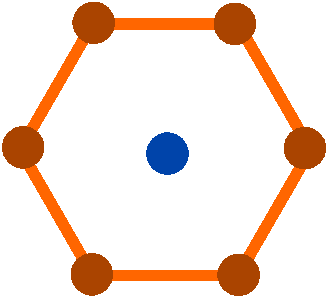
\includegraphics[scale=0.8]{chapter4-outilPoint6-pstricks}
  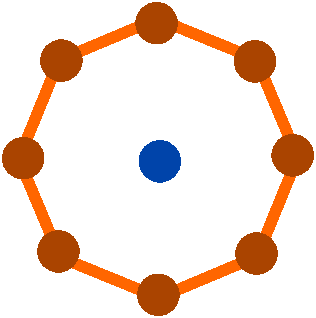
\includegraphics[scale=0.8]{chapter4-outilPoint8-pstricks}

  \caption[Cages d'influence à partir d'un point] {Différentes cages
d'influence créées à partir d'un point comme outil de contrôle}
  \label{EXTPoi}

\end{center}
\end{figure}

Dans le même esprit, nous pourrions obtenir une cage d'influence à partir
d'une courbe. La cage d'influence pourrait être générée comme un
épaississement de la courbe. Le lien entre la courbe et la cage d'influence
pourrait se faire comme pour les cages de contrôle. Mis à part qu'ici au lieu
de modifier la position d'un seul sommet, un point de contrôle modifierait la
position des deux sommets qui résultent de l'épaissement de la courbe au niveau
de ce point de contrôle (Figure \ref{EXTCou}).

\begin{figure}[ht]
\begin{center}
  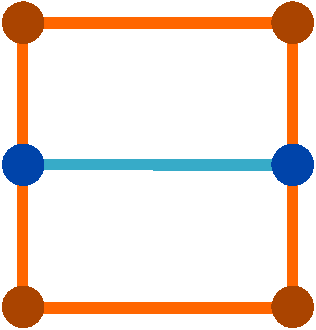
\includegraphics[scale=0.8]{chapter4-outilCourbe4-pstricks}
  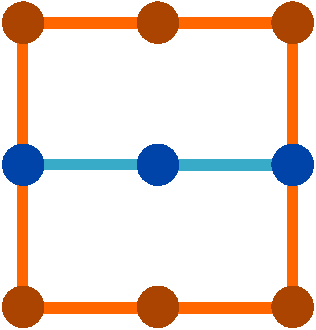
\includegraphics[scale=0.8]{chapter4-outilCourbe6-pstricks}
  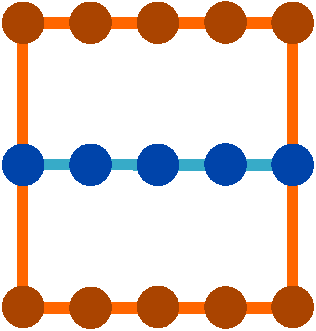
\includegraphics[scale=0.8]{chapter4-outilCourbe10-pstricks}

  \caption[Cages d'influence à partir d'une courbe] {Différentes cages
d'influence créées à partir de courbes de différentes résolutions comme outils
de contrôle}

  \label{EXTCou}

\end{center}
\end{figure}

\section{Mélange d'outils existants}

Plusieurs outils existent déjà, comme nous avons pu le voir dans le chapitre
qui fait l'état de l'art des outils de différentes dimensions. On se demande
alors si notre technique peut se mélanger avec des outils de différentes
dimensions (points ou courbes). Et si c'est possible, comment notre technique
pourrait permettre de mélanger ces différents outils ensemble.

Un point important de la méthode de mélange proposée dans ce travail est la
notion de \textit{distance à l'outil}. En effet, c'est grâce à cette distance
que l'importance de l'atténuation peut être évaluée. A partir du moment où un
outil permet de connaître la position d'un point de l'espace par rapport à la
position des points de contrôle de cet outil et au bord du domaine
d'influence, la technique de mélange présentée au chapitre précédent devrait
fonctionner.

Il est évident que les outils de déformation dont l'influence est globale ne
peuvent pas être utilisés tels quels, car ils n'ont pas un domaine d'influence
fini. Néanmoins, comme nous l'avons fait pour les déformations à base de
cages, il devrait être possible de rendre leur influence locale. Une fois le
domaine d'influence défini, il serait possible d'évaluer le critère de
"distance à l'outil". Cette distance calculée nous permettrait de mélanger ces
outils avec les autres outils tenant aussi compte de la distance à l'outil.

Ces réflexions sont purement théoriques et certaines suppositions pourraient
être fausses, néanmoins nous pensons que des réflexions plus poussées dans ces
directions seraient intéressantes pour les travaux futurs.
